\qrchapter{https://forgottenpillar.com/rsc/en-fp-chapter12}{Heaven's reality}


\qrchapter{https://forgottenpillar.com/rsc/es-fp-chapter12}{La realidad del cielo}


The \emcap{personality of God} deals with the quality or state of God being a person. Whenever we look at the pioneer's work on the \emcap{personality of God}, we see that they were all in harmony with the view that God is a tangible \textit{being}, possessing both body and parts. We always see the same underlying reasoning, which differentiates the term ‘\textit{spirit}’ and the term ‘\textit{being}’. By differentiating these terms, they explain the quality or state of God being a person\footnote{\href{https://www.merriam-webster.com/dictionary/personality}{Merriam-Webster Dictionary} defines the word ‘\textit{personality}’ as “\textit{quality or state of being a person}”.}—a \emcap{personality of God}. All their conclusions are summed up in the first point of the \emcap{Fundamental Principles}. \others{There is \textbf{one God}, a \textbf{personal}, \textbf{spiritual being}, the Creator of all things, omnipotent, omniscient, … and \textbf{every-where present by his representative, the Holy Spirit}. Psalm 139:7.}[FPSDA 1.2][https://egwwritings.org/read?panels=p1299.6]


La \emcap{personalidad de Dios} trata de la cualidad o estado de Dios siendo una persona. Siempre que observamos la obra de los pioneros sobre la \emcap{personalidad de Dios}, vemos que todos ellos estaban en armonía con la opinión de que Dios es un \textit{ser} tangible, que posee cuerpo y partes. Siempre vemos el mismo razonamiento subyacente, que diferencia el término ‘\textit{espíritu}’ y el término ‘\textit{ser}’. Al diferenciar estos términos, explican la cualidad o estado de Dios siendo una persona\footnote{\href{https://www.merriam-webster.com/dictionary/personality}{El Diccionario Merriam-Webster} define la palabra ‘\textit{personalidad}’ como “\textit{cualidad o estado de ser una persona}”.}—una \emcap{personalidad de Dios}. Todas sus conclusiones se resumen en el primer punto de los \emcap{Principios Fundamentales}. \others{Hay \textbf{un solo Dios}, un \textbf{ser personal}, \textbf{espiritual}, creador de todas las cosas, omnipotente, omnisciente, … y \textbf{presente en todas partes por su representante, el Espíritu Santo}. Salmo 139:7.}[FPSDA 1.2][https://egwwritings.org/read?panels=p1299.6]


So far, in the pioneers’ work, we have seen that the \emcap{personality of God} is tightly connected to the reality of God’s presence. God is a personal spiritual being, having a body and shape; as such, His presence is cumbered to one locality—as the Bible says, in His temple, at His throne where He is surrounded with unapproachable glory. But He is everywhere present by His representative, the Holy Spirit. Obviously, the Holy Spirit is a spirit, and not a being, \bible{for a spirit hath not flesh and bones as ye see me have}, said Jesus (Luke 24:39). Christ is also a Being, like His Father. He is an express image of the Father’s person; therefore, He bears the same personality, or the quality or state of being a person, as His Father does.


Hasta ahora, en el trabajo de los pioneros, hemos visto que la \emcap{personalidad de Dios} está estrechamente relacionada con la realidad de la presencia de Dios. Dios es un ser espiritual personal, que tiene un cuerpo y una forma; como tal, su presencia está acumulada en un lugar—como dice la Biblia, en su templo, en su trono, donde está rodeado de una gloria inaccesible. Pero está presente en todas partes por medio de su representante, el Espíritu Santo. Obviamente, el Espíritu Santo es un espíritu, y no un ser, \bible{porque un espíritu no tiene carne ni huesos como veis que tengo yo}, dijo Jesús (Lucas 24:39). Cristo también es un Ser, como su Padre. Es una imagen expresa de la persona del Padre; por lo tanto, tiene la misma personalidad, o cualidad o estado de ser persona, que tiene su Padre.


In our experience, when we present the original Seventh-day Adventist beliefs on the \emcap{personality of God} to our trinitarian brothers, as expressed in the first two points of the \emcap{Fundamental Principles}, they often claim that the statements in the \emcap{Fundamental Principles} are correct in some way, but the understanding attributed to the terms “\textit{personal spiritual being}” are false. They usually attempt to harmonize the \emcap{Fundamental Principles} with the Trinity doctrine by twisting the words “\textit{spiritual being}”, as if the word ‘\textit{spiritual}’ means something mysterious, suitable to equalize the \emcap{personality of God} and of Christ with the personality of the Holy Ghost\footnote{The quality or state of the Holy Spirit being a person is bearing witness, not having the form of a person. \egw{\textbf{The Holy Spirit has a personality}, \textbf{\underline{else} He could not \underline{bear witness} to our spirits} and with our spirits that we are the children of God. \textbf{He must also be a divine person}, \textbf{\underline{else} He could not \underline{search out} the secrets which lie hidden in the mind of God}. ‘For what man knoweth the things of a man save the spirit of man, which is in him; even so the things of God knoweth no man, but the Spirit of God.’ [1 Corinthians 2:11.]}[21LtMs, Ms 20, 1906, par. 32][https://egwwritings.org/read?panels=p14071.10296041&index=0]. It is crystal clear that the Holy Spirit is a person, yet not in the same way as the Father and the Son, as the Holy Spirit does not possess the quality of an outward physical personage like the Father and the Son do.}. The underlying problem comes down to the understanding of the heavenly realities. The Bible is not silent about heaven, and its realities, and our pioneers understood it well. Below we read about the explanation of the terms “\textit{spiritual being}” from James White and Uriah Smith in their book, “\textit{The Biblical Institute}”. The Bible explains these terms using the example of angels, which are “\textit{spiritual beings}”.


Según nuestra experiencia, cuando presentamos a nuestros hermanos trinitarios las creencias originales de los Adventistas del Séptimo Día sobre la \emcap{personalidad de Dios}, tal como se expresan en los dos primeros puntos de los \emcap{Principios Fundamentales}, a menudo afirman que las declaraciones de los \emcap{Principios Fundamentales} son correctas en cierto modo, pero que el entendimiento atribuido a los términos “\textit{ser espiritual personal}” es falso. Suelen intentar armonizar los \emcap{Principios Fundamentales} con la doctrina trinitaria tergiversando las palabras “\textit{ser espiritual}”, como si la palabra ‘\textit{espiritual}’ significara algo misterioso, adecuado para igualar la \emcap{personalidad de Dios} y de Cristo con la personalidad del Espíritu Santo\footnote{La cualidad o estado del Espíritu Santo siendo una persona es dar testimonio, no tener la forma de una persona. \egw{\textbf{El Espíritu Santo tiene una personalidad}, \textbf{\underline{de lo contrario} no podría \underline{dar testimonio} a nuestros espíritus} y con nuestros espíritus de que somos hijos de Dios. \textbf{También debe ser una persona divina}, \textbf{\underline{de lo contrario} no podría \underline{escudriñar} los secretos que están ocultos en la mente de Dios}. ‘Porque ¿quién de los hombres sabe las cosas del hombre, sino el espíritu del hombre que está en él? Así tampoco nadie conoció las cosas de Dios, sino el Espíritu de Dios.’ [1 Corintios 2:11.]}[21LtMs, Ms 20, 1906, par. 32][https://egwwritings.org/read?panels=p14071.10296041&index=0]. Es cristalino que el Espíritu Santo es una persona, pero no de la misma manera que el Padre y el Hijo, ya que el Espíritu Santo no posee la cualidad de un personaje físico exterior como lo hacen el Padre y el Hijo.}. El problema de fondo se reduce a la comprensión de las realidades celestiales. La Biblia no guarda silencio sobre el cielo y sus realidades, y nuestros pioneros lo entendieron bien. A continuación leemos la explicación de los términos “\textit{ser espiritual}” de James White y Uriah Smith en su libro, “\textit{The Biblical Institute}”. La Biblia explica estos términos utilizando el ejemplo de los ángeles, que son “\textit{seres espirituales}”.


\begin{figure}[hp]
    \centering
    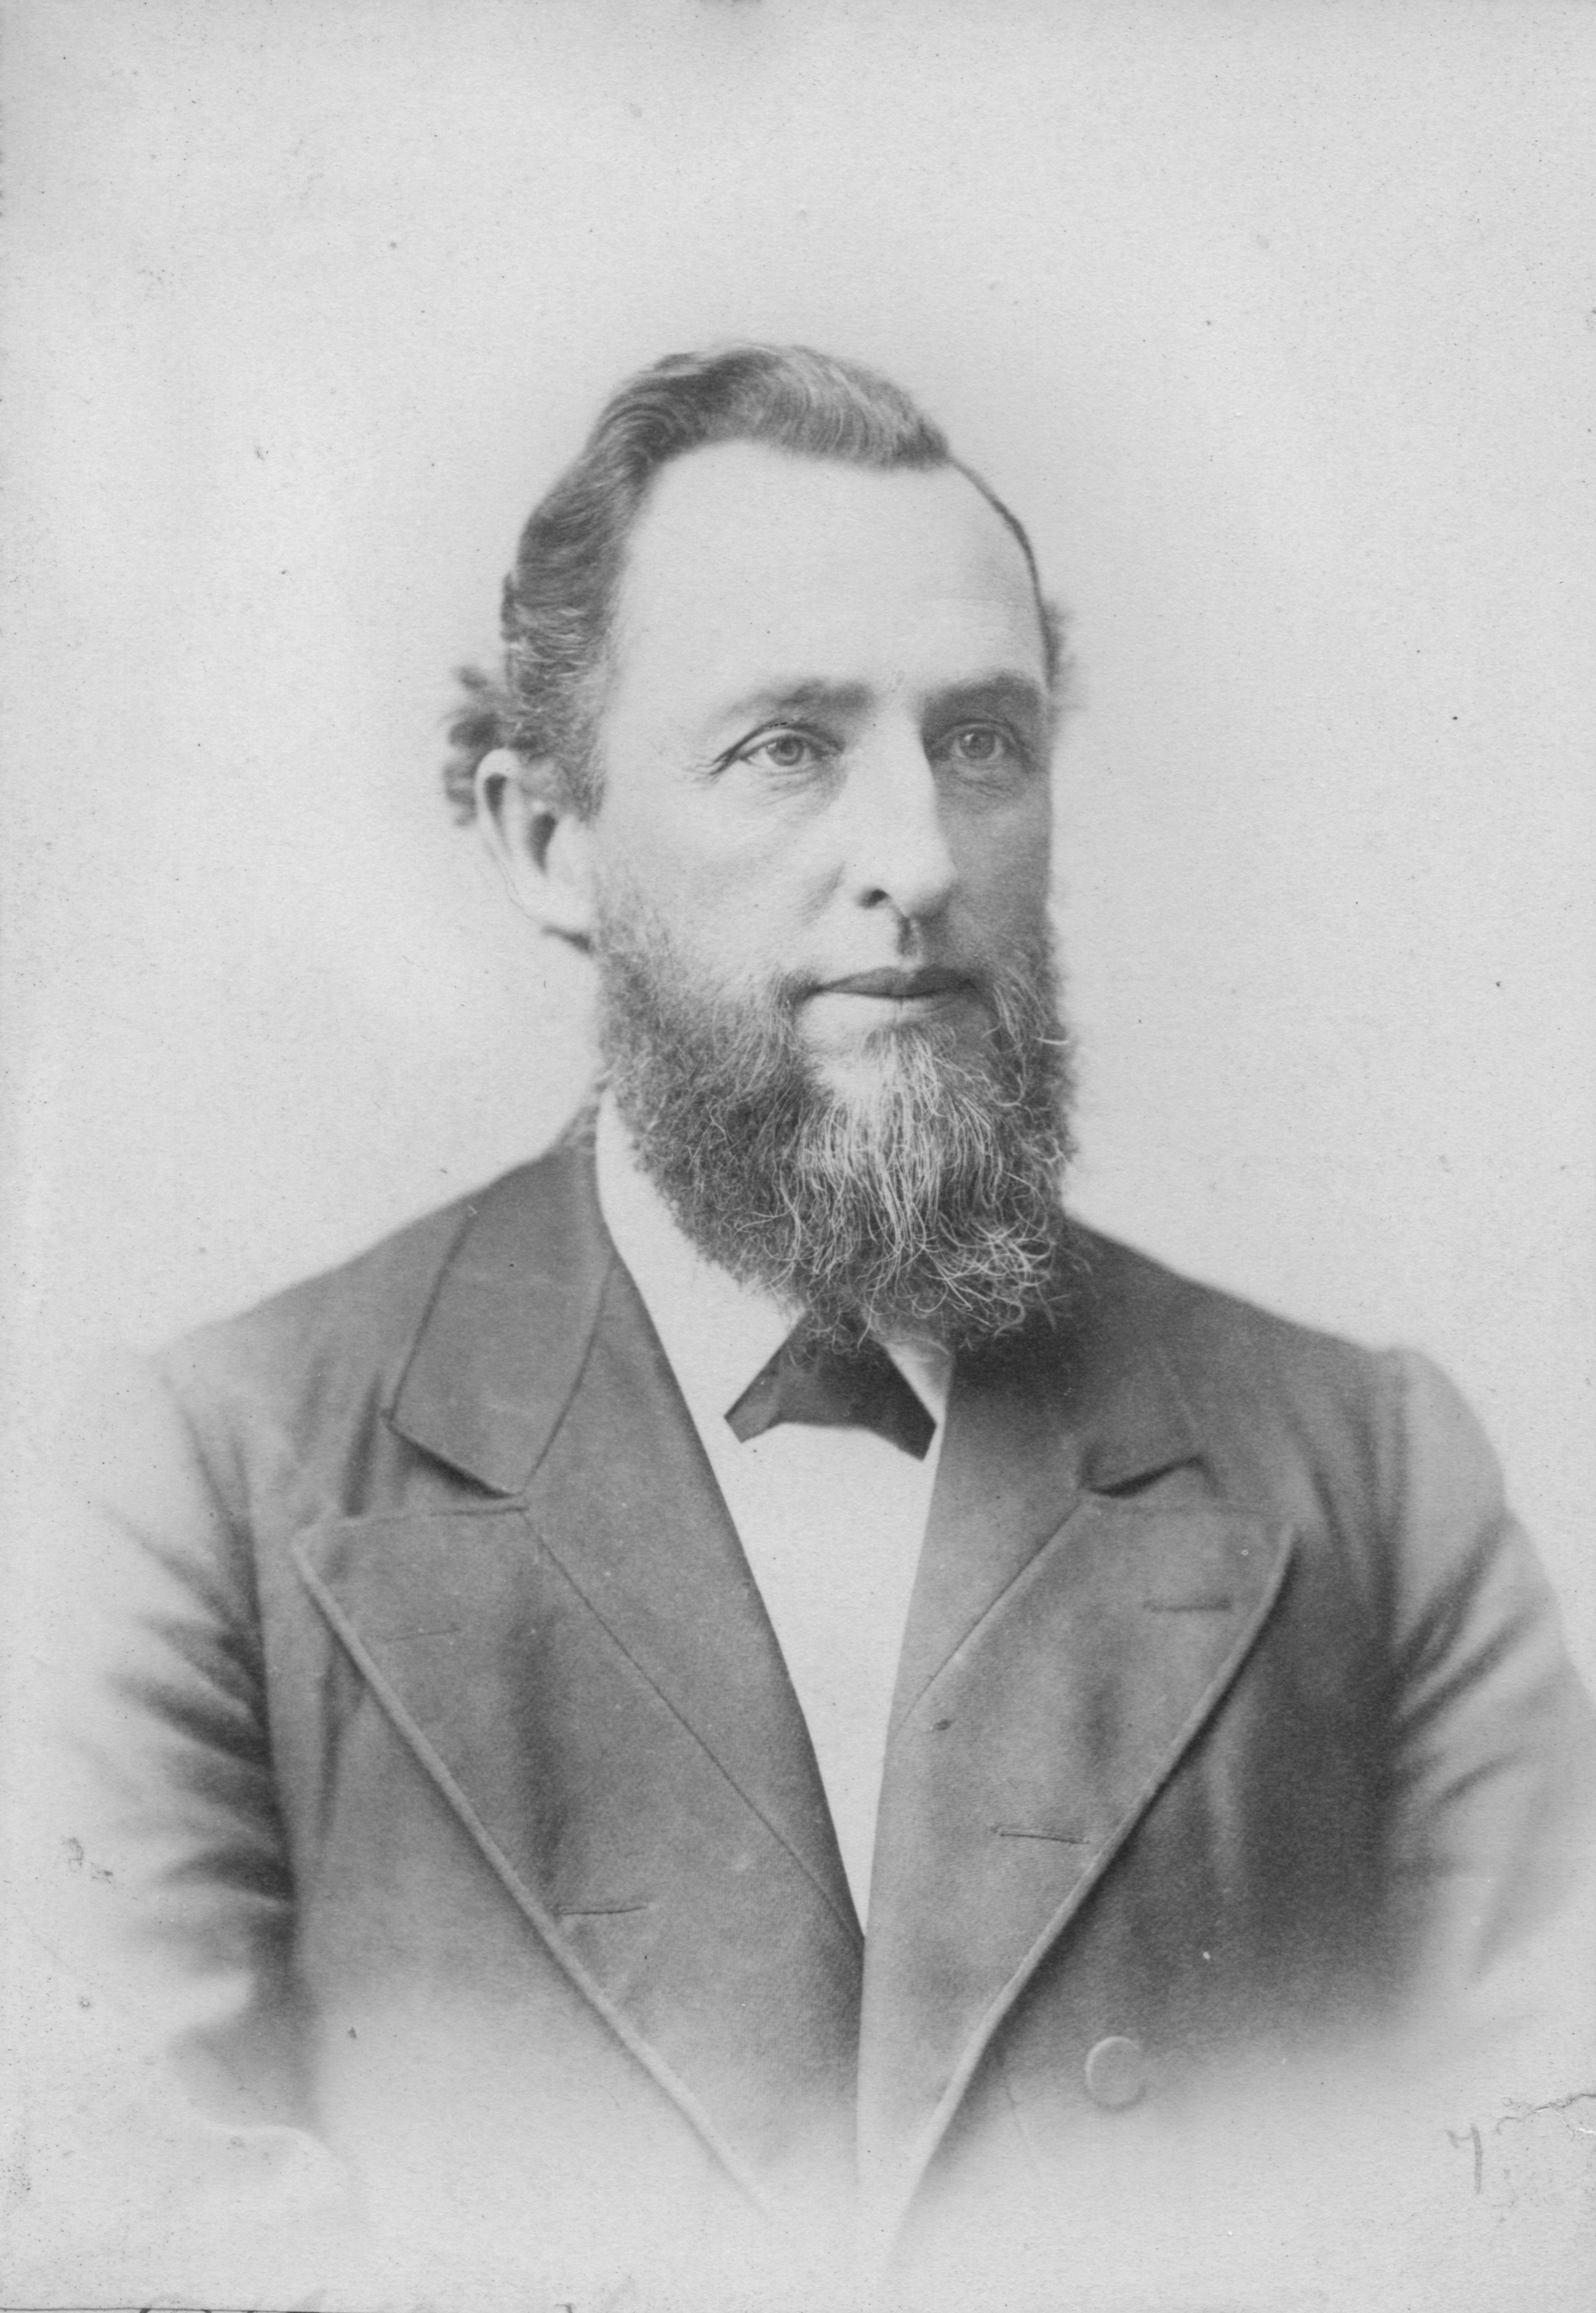
\includegraphics[width=1\linewidth]{images/uriah-smith.jpg}
    \caption*{Uriah Smith (1832-1903)}
    \label{fig:uriah-smith}
\end{figure}


\begin{figure}[hp]
    \centering
    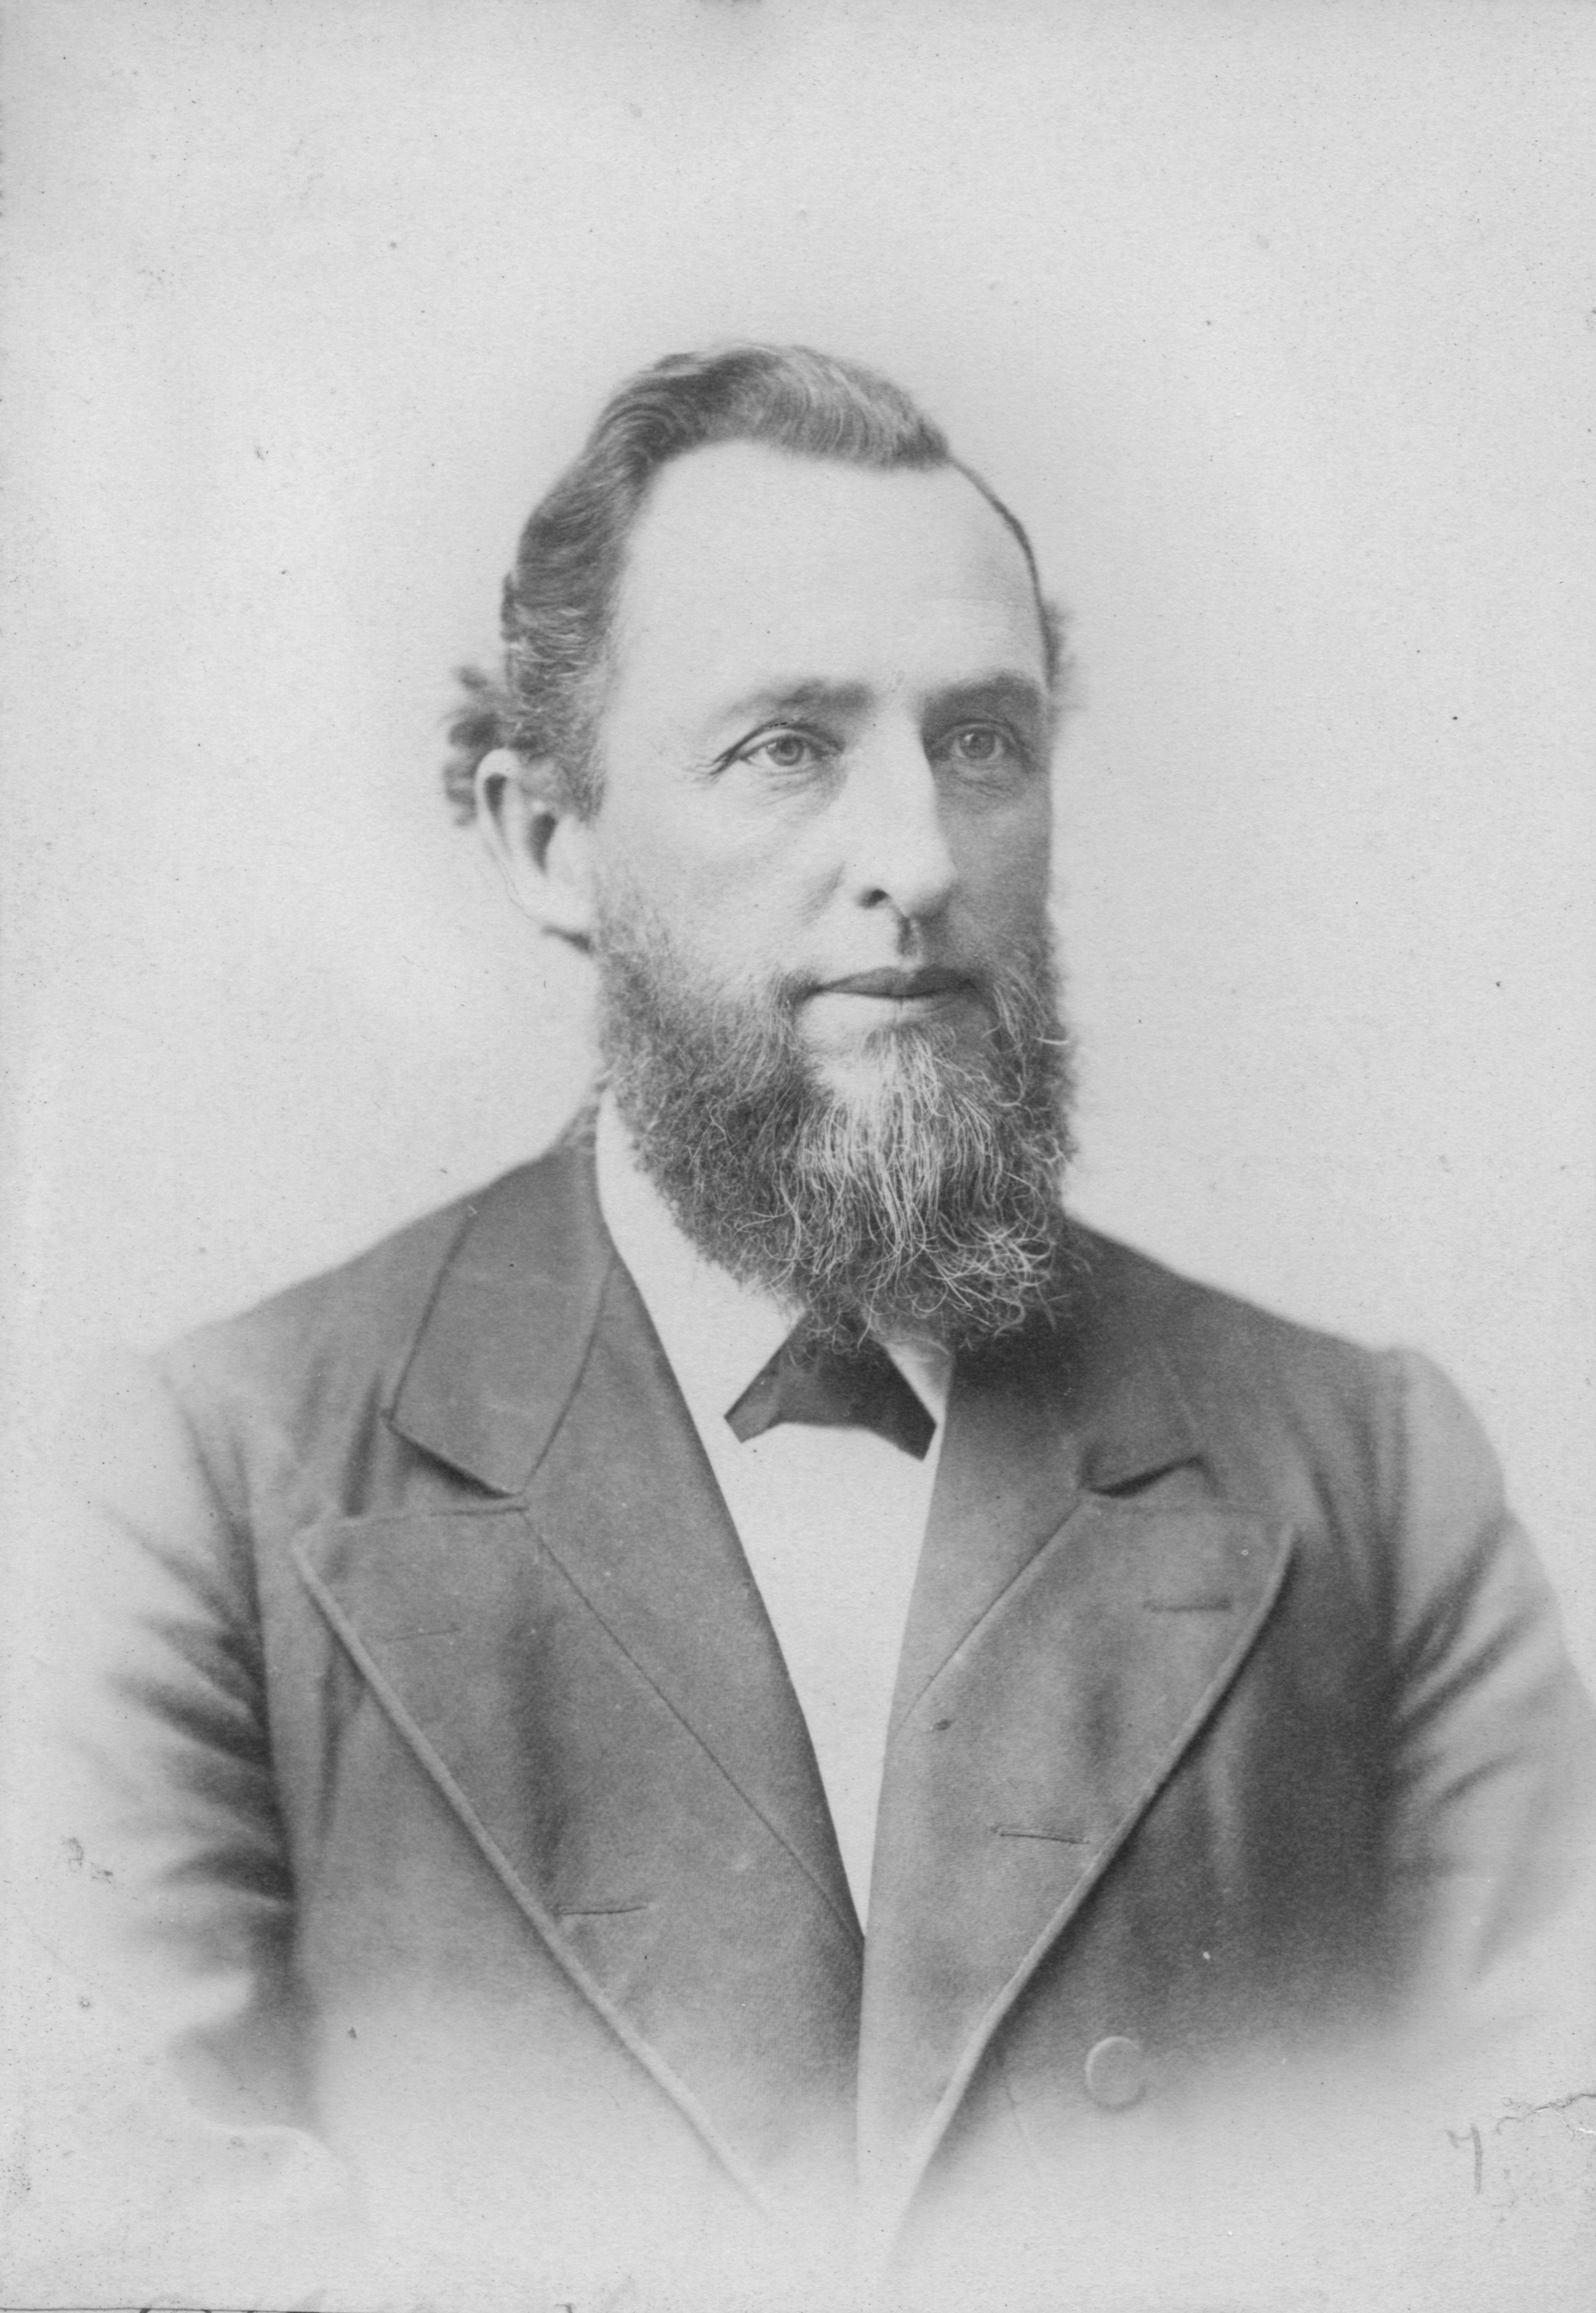
\includegraphics[width=1\linewidth]{images/uriah-smith.jpg}
    \caption*{Uriah Smith (1832-1903)}
    \label{fig:uriah-smith}
\end{figure}


\others{\textbf{Angels are real beings}. They are described in the Bible as \textbf{possessing face, feet, wings} \&x. Ezekiel says of the cherubim, ‘\textbf{Their whole \underline{body} and their backs and their hands and their wings},’ \&c. Eze. 10:12. Angels \textbf{appeared }unto Abraham. Gen. 18:1-8. They talked and ate with him. They went on to Sodom and communed with Lot, who, entering into his house baked unleavened bread for them and they did eat. \textbf{These person were called angels}. David speaks of the manna as the corn of Heaven and angel’s food. Ps. 78:23-25.}


\others{\textbf{Los ángeles son seres reales}. Se describen en la Biblia como \textbf{poseedores de rostro, pies, alas} \&x. Ezequiel dice de los querubines, ‘\textbf{Todo su \underline{cuerpo}, sus espaldas, sus manos, sus alas},’ \&c. Eze. 10:12. Los ángeles \textbf{se le aparecieron} a Abraham. Gn. 18:1-8. Hablaron y comieron con él. Siguieron hasta Sodoma y estuvieron en comunión con Lot, quien, al entrar en su casa, les horneó panes sin levadura y comieron. \textbf{Estas personas fueron llamadas ángeles}. David habla del maná como el maíz del cielo y el alimento de los ángeles. Salmo 78:23-25.}


\othersnogap{The case of Balaam, Num. 22:22-31, is an interesting incident. The angel \textbf{appeared }to Balaam with a sword \textbf{drawn in his hand}. The question is sometimes asked \textbf{how angels can be \underline{material beings since we cannot see them}. This case illustrates it}. The record says the \textbf{Lord opened the eyes of Balaam and he saw the angel}. \textbf{The angel did not create a body for that occasion}.\textbf{ He was just the same as he was before Balaam saw him; \underline{but the change took place in Balaam}. His eyes were opened, then he beheld the angel}. It was the same with the servant of Elisha when he and his master were brought into a straight place, surrounded by the army of the king of Syria. 2 Kings 6:17. Elisha prayed that \textbf{the eyes of his servant might be opened}; and he immediately saw the whole mountain full of horses and chariots round about Elisha.}


\othersnogap{El caso de Balaam, Núm. 22:22-31, es un incidente interesante. El ángel \textbf{se le apareció} a Balaam con una espada \textbf{desenvainada en la mano}. A veces se pregunta \textbf{cómo los ángeles pueden ser \underline{seres materiales, ya que no podemos verlos}. Este caso lo ilustra}. El registro dice que el \textbf{Señor abrió los ojos de Balaam y él vio al ángel}. \textbf{El ángel no creó un cuerpo para esa ocasión}. \textbf{Era igual que antes de que Balaam lo viera; \underline{pero el cambio tuvo lugar en Balaam}. Sus ojos se abrieron y entonces vio al ángel}. Lo mismo ocurrió con el siervo de Eliseo cuando él y su amo fueron llevados a un lugar recto, rodeados por el ejército del rey de Siria. 2 Reyes 6:17. Eliseo oró para que \textbf{se abrieran los ojos de su siervo}; e inmediatamente vio toda la montaña llena de caballos y carros alrededor de Eliseo.}


\othersnogap{\textbf{This may be further illustrated referring to things which we know are material and yet which we cannot see}. Air is material, light is material, even thought itself is only the result of material organizations — matter acting upon matter — and yet we can see none of these things. \textbf{Just so with the angels}.}


\othersnogap{\textbf{Esto puede ilustrarse aún más refiriéndose a las cosas que sabemos que son materiales y que, sin embargo, no podemos ver}. El aire es material, la luz es material, incluso el propio pensamiento es sólo el resultado de organizaciones materiales —materia actuando sobre materia— y, sin embargo, no podemos ver ninguna de estas cosas. \textbf{Lo mismo ocurre con los ángeles}.}


\othersnogap{\textbf{It is further objected to the materiality of the angels that they are called spirits. }Heb. 1:13, 14.\textbf{\underline{But this is no objection to their being literal beings}}. \textbf{They are simply spiritual beings organized differently from these earthly bodies which we possess}. Paul says, 1 Cor. 15:44, ‘\textbf{There is a natural body and there is \underline{a spiritual body}}.’ \textbf{The natural body we now have; the spiritual body we shall have in the resurrection}. ‘\textbf{It is raised a spiritual body}.’ Verse 44. \textbf{But then we are equal unto the angels}, Luke 20:36; \textbf{then we have bodies like unto Christ’s most glorious body}. Phil. 3:4\footnote{Typo: It should be Philippians 3:21} \textbf{and Christ is no less a spirit than the angels}. \textbf{We read that God is a spirit, that is, simply \underline{a spiritual being}}.}[James White and Uriah Smith, The Biblical Institute (Kindle Locations 2537-2553). Kindle Edition.]


\othersnogap{\textbf{Se objeta además a la materialidad de los ángeles que se les llama espíritus. }Heb. 1:13, 14. \textbf{\underline{Pero esto no es una objeción a que sean seres literales}}. \textbf{Son simplemente seres espirituales organizados de manera diferente a estos cuerpos terrenales que poseemos}. Pablo dice, 1 Cor. 15:44, ‘\textbf{Hay cuerpo animal [natural] y hay \underline{cuerpo espiritual}}’. \textbf{El cuerpo natural lo tenemos ahora; el cuerpo espiritual lo tendremos en la resurrección}. ‘\textbf{Resucitará cuerpo espiritual}’. Versículo 44. \textbf{Pero entonces somos iguales a los ángeles}, Lucas 20:36; \textbf{entonces tenemos cuerpos semejantes al cuerpo glorioso de Cristo}. Fil. 3:4\footnote{Error tipográfico: Debería ser Filipenses 3:21} \textbf{y Cristo no es menos espíritu que los ángeles}. \textbf{Leemos que Dios es un espíritu, es decir, simplemente \underline{un ser espiritual}}.}[James White and Uriah Smith, The Biblical Institute (Kindle Locations 2537-2553). Kindle Edition.]


The Bible gives us the insight that angels are spiritual beings that possess material bodies, but are still unseen to us, unless the Lord opens our eyes to see them. When the righteous will rise up in their new glorified bodies, they will rise in a spiritual body, an incorruptible one. This body will be tangible and material just as the new Earth will be tangible and material. And with our spiritual bodies we will possess the renewed Earth, we will replenish it \bible{and subdue it: and have dominion over the fish of the sea, and over the fowl of the air, and over every living thing that moveth upon the earth}[Genesis 1:28].


La Biblia nos da a entender que los ángeles son seres espirituales que poseen cuerpos materiales, pero que siguen sin ser vistos por nosotros, a menos que el Señor abra nuestros ojos para verlos. Cuando los justos se levanten en sus nuevos cuerpos glorificados, lo harán en un cuerpo espiritual, incorruptible. Este cuerpo será tangible y material al igual que la nueva Tierra será tangible y material. Y con nuestros cuerpos espirituales poseeremos la Tierra renovada, la repondremos \bible{y la someteremos, y tendremos dominio sobre los peces del mar, sobre las aves del cielo y sobre todo ser viviente que se mueve sobre la tierra}[Génesis 1:28].


% Heaven's reality

\begin{titledpoem}
    
    \stanza{
        God is not vapor, nor mystery unknown, \\
        A personal being upon Heaven's throne. \\
        Bound by space as a being must, \\
        Yet present through His Spirit's trust.
    }

    \stanza{
        Christ bears His image, a tangible Son, \\
        Two divine beings, not mystically one. \\
        Angels around them with bodies unseen, \\
        Material creatures of heavenly sheen.
    }

    \stanza{
        Our eyes cannot witness their spiritual frame, \\
        Until God reveals what our vision can't claim. \\
        In resurrection we'll rise like them too, \\
        Spiritual bodies, yet tangible and true.
    }

    \stanza{
        Not three equal persons in mystical blend, \\
        But Father and Son with Spirit they send. \\
        The divine is not distant, abstract, or obscure, \\
        But personal, present, and perfectly sure.
    }
    
\end{titledpoem}

% \chapter{Realnost Neba}

\emcap{Ličnost Boga} se bavi kvalitetom ili stanjem koja Boga čine osobom. Kad god pogledamo spise pionira o \emcap{ličnosti Boga}, vidimo da su svi bili u skladu s pogledom da je Bog opipljivo \textit{biće}, koje posjeduje i tijelo i dijelove. Uvijek vidimo isto temeljno rasuđivanje, koje razlikuje pojam ‘\textit{duh}’ i pojam ‘\textit{biće}’. Razlikujući ove pojmove, oni objašnjavaju kvalitetu ili stanje koja Boga čine osobom\footnote{\href{https://www.merriam-webster.com/dictionary/personality}{Merriam-Webster Dictionary} definira riječ ‘\textit{personality}’ kao “\textit{kvaliteta ili stanje koja nekog čine osobom}”.}—\emcap{ličnost Boga}. Svi njihovi zaključci su sažeti u prvoj točki \emcap{Fundamentalnih Principa}. \others{Postoji \textbf{jedan Bog}, \textbf{osobno}, \textbf{duhovno biće}, Stvoritelj svega, svemoguć, sveznajući, … i \textbf{svugdje prisutan preko svog predstavnika, Svetog Duha}. Psalam 139:7.}[FPSDA 1.2][https://egwwritings.org/read?panels=p1299.6]

Dosad smo u spisima pionira vidjeli da je \emcap{ličnost Boga} usko povezana s realnošću Božje prisutnosti. Bog je osobno duhovno biće, ima tijelo i oblik; te kao takav, Njegova prisutnost je ograničena na jedan lokalitet—kako Biblija kaže, u Njegovom hramu, na Njegovom prijestolju gdje je okružen nepristupačnom slavom. No, On je svuda prisutan preko Svog predstavnika, Svetog Duha. Očito, Sveti Duh je duh, a ne biće, \bible{duh nema tijela i kostiju kao što vidite da ja imam}, rekao je Isus (Luka 24:39). Krist je također Biće, kao i Njegov Otac. On je savršena slika Očeve osobe; stoga nosi jednaku ličnost, ili kvalitetu ili stanje koja ga čine osobom, baš kao i Njegovog Oca.

U našem iskustvu, kada bismo predstavili našoj trinitarnoj braći originalna vjerovanja Adventista Sedmog Dana o \emcap{ličnosti Boga}, kako je izraženo u prve dvije točke \emcap{Fundamentalnih Principa}, često su tvrdili kako su izjave u \emcap{Fundamentalnim Principima} na neki način točne, ali da je razumijevanje pripisano terminima “\textit{osobno duhovno biće}” pogrešno. Obično pokušavaju uskladiti \emcap{Fundamentalne Principe} s doktrinom o Trojstvu izvrćući riječi “\textit{duhovno biće}”, kao da riječ ‘\textit{duhovno}’ znači nešto tajanstveno, prikladno da izjednači \emcap{ličnost Boga} i Krista s ličnošću Svetog Duha\footnote{Kvaliteta ili stanje koje Duha Svetoga čini osobom jest svjedočenje, a ne posjedovanje oblika osobe. \egw{\textbf{Duh Sveti ima osobnost}, \textbf{\underline{inače} ne bi mogao \underline{svjedočiti} našem duhu} i s našim duhom da smo djeca Božja. \textbf{On također mora biti božanska osoba}, \textbf{\underline{inače} ne bi mogao \underline{istražiti} tajne koje leže skrivene u umu Božjem}. ‘Jer tko od ljudi zna što je u čovjeku osim duha čovječjega u njemu? Tako i što je u Bogu, nitko ne zna osim Duha Božjega.’ [1 Korinćanima 2:11.]}[21LtMs, Ms 20, 1906, par. 32][https://egwwritings.org/read?panels=p14071.10296041&index=0]. Kristalno je jasno da je Duh Sveti osoba, ali ne na isti način kao Otac i Sin, jer Duh Sveti ne posjeduje kvalitetu vanjske fizičke ličnosti kao što to imaju Otac i Sin.}. Temeljni problem svodi se na razumijevanje nebeskih stvarnosti. Biblija ne šuti o nebu i njegovim stvarnostima, i naši pioniri su to dobro shvatili. Ispod čitamo o objašnjenju termina “\textit{duhovno biće}” iz knjige Jamesa Whitea i Uriaha Smitha, “\textit{Biblijski Institut}”. Biblija objašnjava te termine koristeći primjer anđela, koji su “\textit{duhovna bića}”.

\others{\textbf{Anđeli su stvarna bića}. U Bibliji su opisani kao oni koji \textbf{posjeduju lice, stopala, krila} itd. Ezekiel kaže za kerubine, ‘\textbf{A cijelo njihovo \underline{tijelo} i leđa njihova i ruke njihove i krila njihova},’ itd. Eze. 10:12. Anđeli su se \textbf{ukazali} Abrahamu. Post. 18:1-8. Razgovarali su i jeli s njim. Otišli su u Sodomu i razgovarali s Lotom, koji je, ušavši u svoju kuću, ispekao beskvasni kruh za njih i oni su jeli. \textbf{Ove osobe su nazivane anđelima}. David govori o mani kao o nebeskom žitu i anđeoskoj hrani. Ps. 78:23-25.}

\othersnogap{Bileamov slučaj, Br. 22:22-31, zanimljiv je događaj. Anđeo se \textbf{ukazao} Bileamu s \textbf{isukanim mačem u ruci}. Ponekad se postavlja pitanje \textbf{kako anđeli mogu biti \underline{materijalna bića kad ih ne možemo vidjeti}. Ovaj slučaj to ilustrira}. Zapis kaže da je \textbf{Gospodin otvorio oči Bileamu i on je ugledao anđela}. \textbf{Anđeo nije stvorio tijelo za tu priliku}. \textbf{Bio je isti kakav je bio prije nego što ga je Bileam ugledao; ali se \underline{promjena dogodila u Bileamu}}. Oči su mu se otvorile, a zatim je ugledao anđela. Isto je bilo s Elizejevim slugom kad su on i njegov gospodar bili dovedeni u dolinu, okruženi vojskom sirijskog kralja. 2. Kraljevima 6:17. Elizej se molio da se \textbf{oči njegova sluge otvore}; i odmah ugleda cijelu planinu punu konja i bojnih kola oko Elizeja.}

\othersnogap{\textbf{Ovo se može dodatno ilustrirati pozivajući se na stvari za koje znamo da su materijalne, a koje ipak ne možemo vidjeti}. Zrak je materijal, svjetlost je materijalna, čak je i sama misao samo rezultat materijalnih organizacija—materija djeluje na materiju—a ipak ne možemo vidjeti ništa od toga. \textbf{Tako je i s anđelima}.}

\othersnogap{\textbf{Nadalje, prigovor za materijalnost anđela je da se nazivaju duhovima}. Hebr. 1:13, 14. \textbf{\underline{Ali to nije prigovor da su oni doslovna bića}}. \textbf{Oni su jednostavno duhovna bića organizirana drugačije od ovih zemaljskih tijela koja posjedujemo}. Pavao kaže, 1 Kor. 15:44, ‘\textbf{Postoji prirodno tijelo i postoji \underline{duhovno tijelo}}.’ \textbf{Prirodno tijelo koje sada imamo; duhovno tijelo koje ćemo imati u uskrsnuću}. ‘\textbf{Ustaje duhovno tijelo}.’ Stih 44. \textbf{Ali tada smo jednaki anđelima}, Luka 20:36; \textbf{tada imamo tijela slična Kristovom najslavnijem tijelu}. Fil. 3:4 \textbf{a Krist nije ništa manje duh od anđela}. \textbf{Čitamo da je Bog duh, to jest jednostavno \underline{duhovno biće}}.}[James White and Uriah Smith, The Biblical Institute (Kindle Lokacija 2537-2553). Kindle Verzija.]

Biblija nam daje uvid da su anđeli duhovna bića koja posjeduju materijalna tijela, ali su nam i dalje nevidljiva, osim ako Gospodin ne otvori naše oči da ih vidimo. Kada pravednici uskrsnu u svojim novim proslavljenim tijelima, uskrsnut će u duhovnom tijelu, nepropadljivom. To tijelo će biti opipljivo i materijalno, baš kao što će Nova Zemlja biti opipljiva i materijalna. I s našim duhovnim tijelima posjedovat ćemo obnovljenu Zemlju: \bible{plodite se i množite i napunite zemlju, i sebi je podložite! I budite gospodari ribama morskim i pticama nebeskim i svemu živomu što gmiže po zemlji!}[Postanak 1:28].

% Stvarnost Neba

\begin{titledpoem}
    \stanza{
        Bog nije tajna ni nestvarna sila, \\
        Već biće stvarno što nebo je svila. \\
        Tijelo i oblik On zaista ima, \\
        Na prijestolju sjedi, vidljiv anđelima.
    }

    \stanza{
        Duhovno biće, ali ipak stvarno, \\
        Prisutan svugdje, ali ne proizvoljno. \\
        Kroz Svetoga Duha svugdje djeluje, \\
        Predstavnik Njegov svijetom putuje.
    }

    \stanza{
        Sin slika Oca, iste naravi, \\
        Obojica bića u stvarnoj pojavi. \\
        Anđeli također tijela imaju, \\
        Iako se našim očima ne daju.
    }

    \stanza{
        U uskrsnuću i mi ćemo biti, \\
        Poput anđela, duhovna tijela zadobiti. \\
        Tijela duhovna, ali opipljiva, \\
        Na Zemlji novoj, stvarnoj i predivnoj.
    }
\end{titledpoem}


